\section{Paper 3}
\subsection{\emph{"An End-to-End Compression Framework Based on Convolutional Neural Networks"}}

\begin{frame}{INTRODUCTION}
    In recent years, within the field of computer vision, remarkable results 
    have been achieved with regard to image compression. The purpose of 
    compressionis to be able to transmit, or save, the entire image at low bit 
    rates. The following article presents a compression method based on 
    convolutional neural networks (CNNs) which, through the use of various 
    state-of-the-art codecs, are able to achieve better performance in terms 
    of compression and image quality.
\end{frame}

\begin{frame}{RELATED WORK}
    At the state of the art there are post-processing methods that use 
    {\bfseries{deblocking}} and {\bfseries{restoring}} techniques \footfullcite{0799924108}. These techniques have a strong 
    computational impact on systems. These operations focus on eliminating 
    artifacts and blocks that contain noise within the image. Other methods 
    use CNNs for {\bfseries{super-resolution}} (SR) images \footfullcite{0799924123}. There are deep learning 
    methods that are used for {\bfseries{lossy}} \footfullcite{0799924125} or {\bfseries{lossless}} \footfullcite{0799924130} compression of images, but 
    these ignore the use of the various existing codecs.
\end{frame}

\begin{frame}{THE PROPOSED COMPRESSION FRAMEWORK pt1}
    The proposed system is composed of two convolutional neural networks:
    \begin{enumerate}
        \item \emph{ComCNN}: used for compact representation of images
        \item \emph{RecCNN}: used for decoding and reconstruction of images
    \end{enumerate}
    \begin{figure}[htbp]
        \centering
        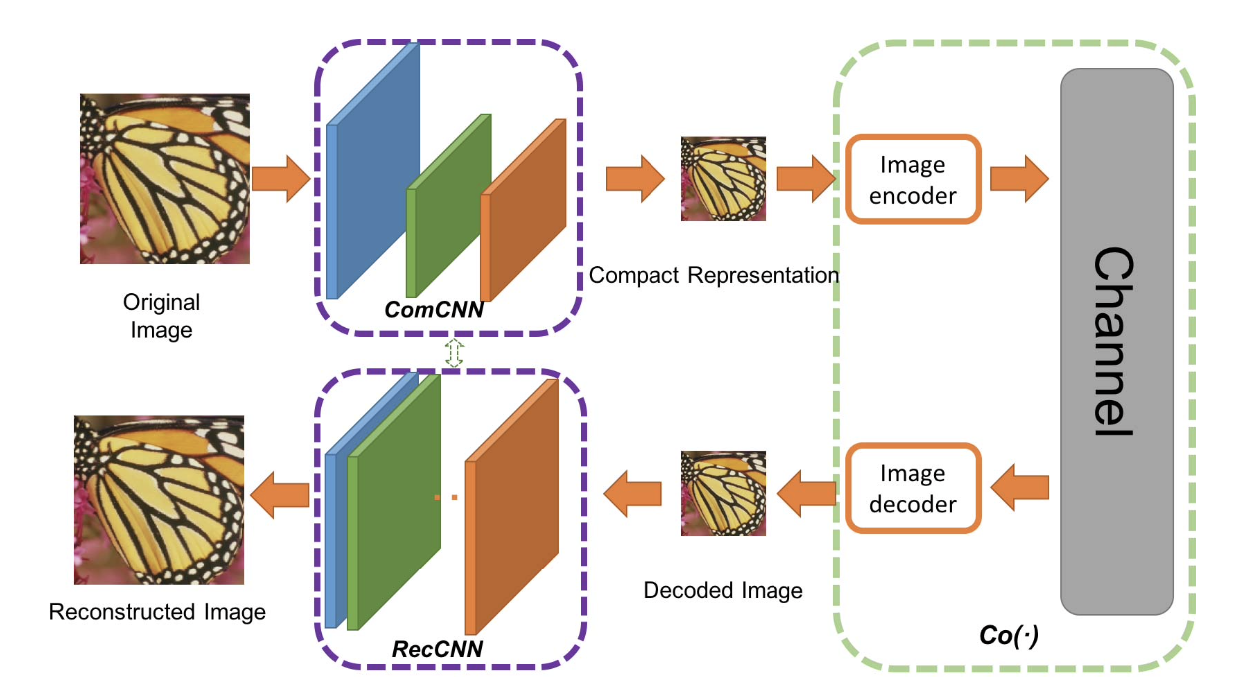
\includegraphics[width = 0.8 \linewidth]{images/paper3/framework.png}
        \centering
        \caption{Up: the ComCNN. Down: the RecCNN. Right: the codec.}
        \label{fig: framework}
    \end{figure}
\end{frame}

\begin{frame}{THE PROPOSED COMPRESSION FRAMEWORK pt2}
    \begin{minipage}{\linewidth}
        \centering
        \begin{minipage}{0.45\linewidth}
            \begin{figure}[H]
                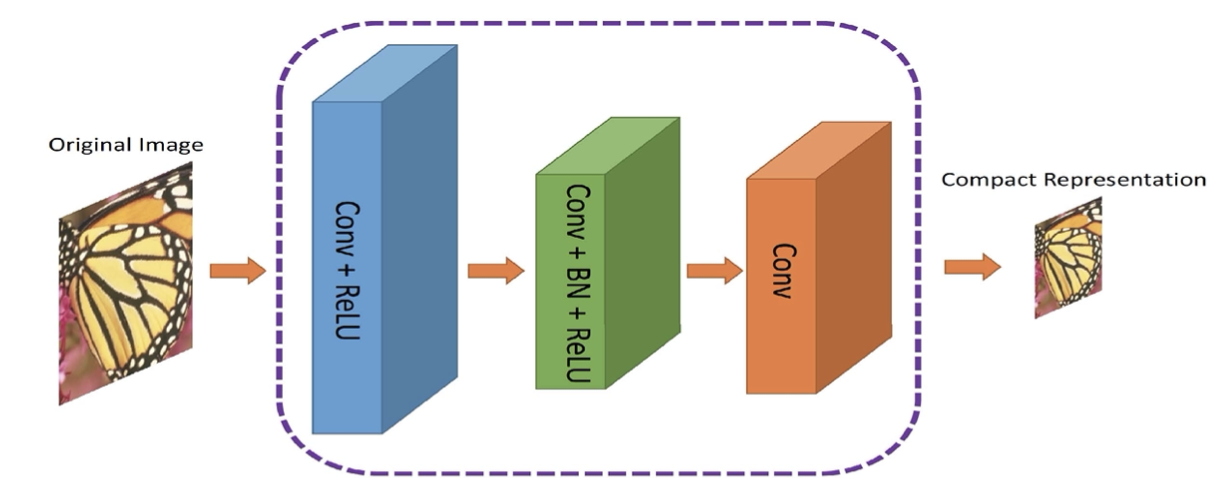
\includegraphics[width = 1 \linewidth]{images/paper3/ComCNN.png}
                \caption{ComCNN architecture.}
            \end{figure}
            \begin{block}{Parameter optimizations}
                \small $$ \hat{\theta_1} = \argmin\limits_{\theta_1}||Re(\hat{\theta_2},Cr(\theta_1,x))-x||^2 $$
            \end{block}
            \begin{block}{Loss Function}
               \tiny $$ L_1(\theta_1) = \frac{1}{2N}\sum_{k=1}^N||Re(\hat{\theta_2}, C_r(\theta1,x_k))-x_k||^2 $$
            \end{block}
        \end{minipage}
        \hspace{0.05\linewidth}
        \begin{minipage}{0.45\linewidth}
            \begin{figure}[htbp]
                \centering
                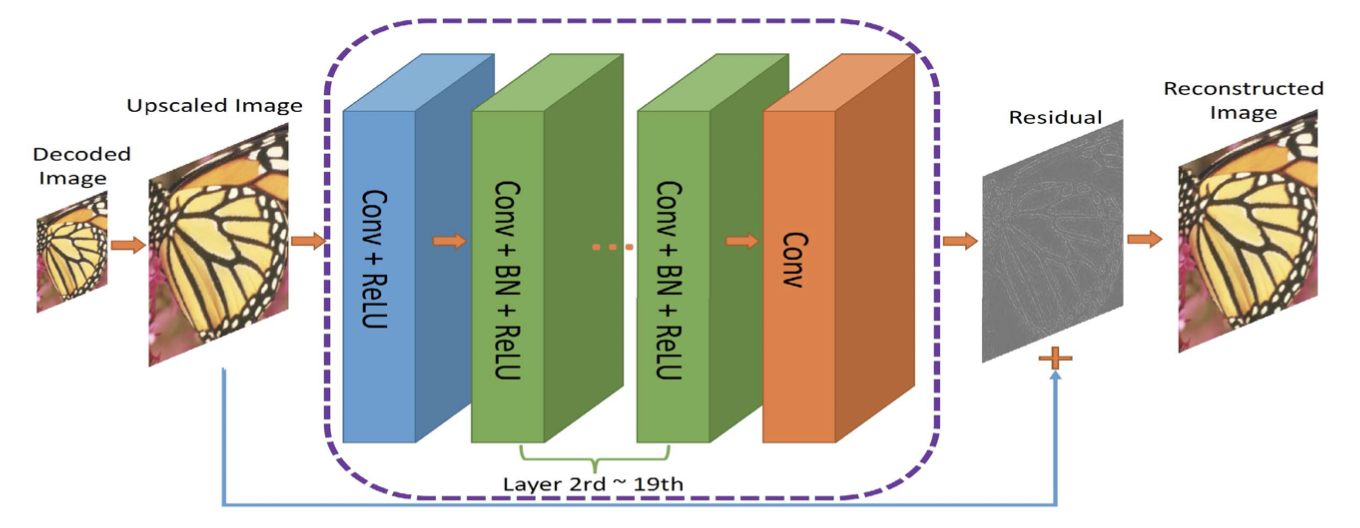
\includegraphics[width = 1 \linewidth]{images/paper3/RecCNN.png}
                \centering
                \caption{RecCNN architecture.}
            \end{figure}
            \begin{block}{Parameter optimizations}
                \small $$ \hat{\theta_2} = \argmin\limits_{\theta_2}||Re(\hat{\theta_2},\hat{x}_m)-x||^2 $$
            \end{block}
            \begin{block}{Loss Function}
                \tiny $$ L_2(\theta_2) = \frac{1}{2N}\sum_{k=1}^N||res(Co(\hat{x}_{mk}), \theta_2) - (Co(\hat{x}_{mk})-x_k)||^2 $$
             \end{block}
        \end{minipage}
    \end{minipage}
\end{frame}

\begin{frame}{EXPERIMENTS}
    The performance comparison is made by citing various techniques present 
    at the state of the art. A compression quality index ({\bfseries\emph{PSNR}}) and ù
    an image similarity index ({\bfseries\emph{SSIM}}) are used. What is really important to note 
    is how the proposed method manages to have better performance than 
    the already used codecs such as \emph{JPEG}, \emph{JPEG2000} and \emph{BPG}, at different 
    bit rates (\emph{bpp}) and quality factors (\emph{QS}). As for the execution times, in 
    terms of CPU / GPU, the proposed algorithm is faster than those already 
    existing.
    \begin{figure}[htbp]
        \centering
        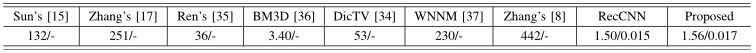
\includegraphics[width = 1 \linewidth]{images/paper3/time.png}
        \centering
        \caption{Running time(s) of compared methods in CPU (/GPU) }
        \label{fig:time}
    \end{figure}
\end{frame}

\begin{frame}{EXPERIMENTS: JPEG vs. The proposed system}
    With a variable QF (first set to 5 and then to 10), the results obtained by 
    the various methods, in terms of PSNR and SSIM, are shown in the following figures:
    \begin{minipage}{\linewidth}
        \centering
        \begin{minipage}{0.45\linewidth}
            \begin{figure}[H]
                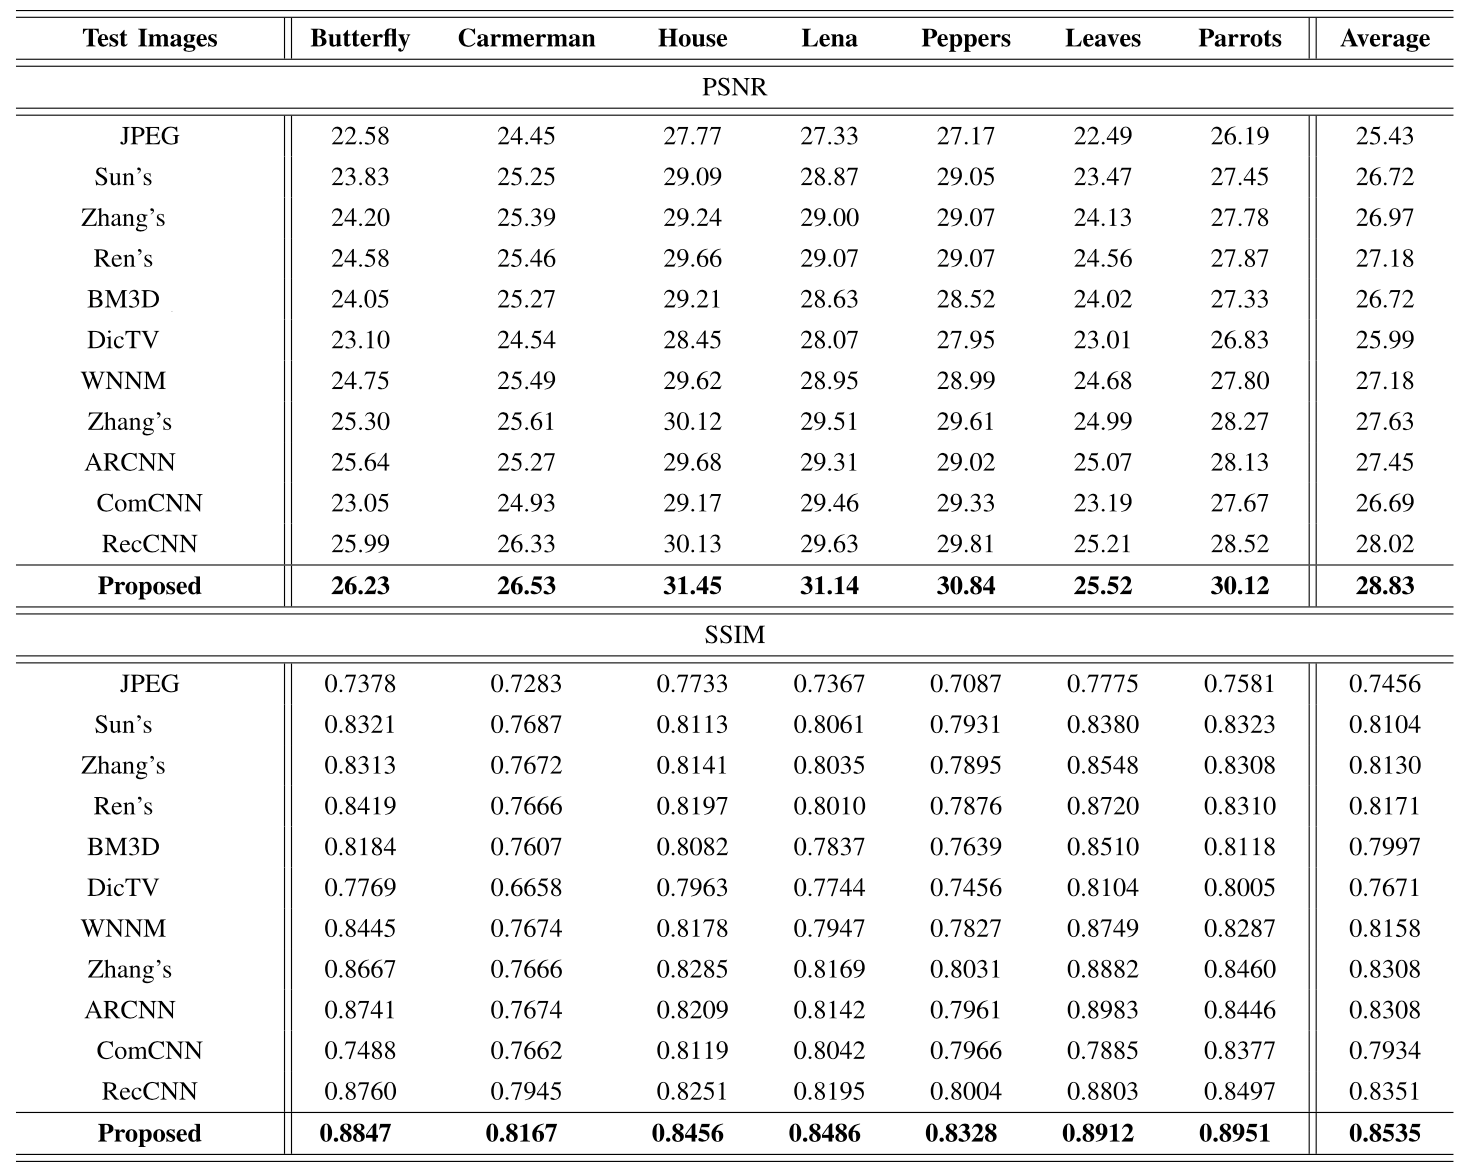
\includegraphics[width = 1 \linewidth]{images/paper3/comparison.png}
                \caption{QF = 5, PSNR(db) and SSIM results of alghoritms image deblocking and denoising}
            \end{figure}
        \end{minipage}
        \hspace{0.05\linewidth}
        \begin{minipage}{0.45\linewidth}
            \begin{figure}[htbp]
                \centering
                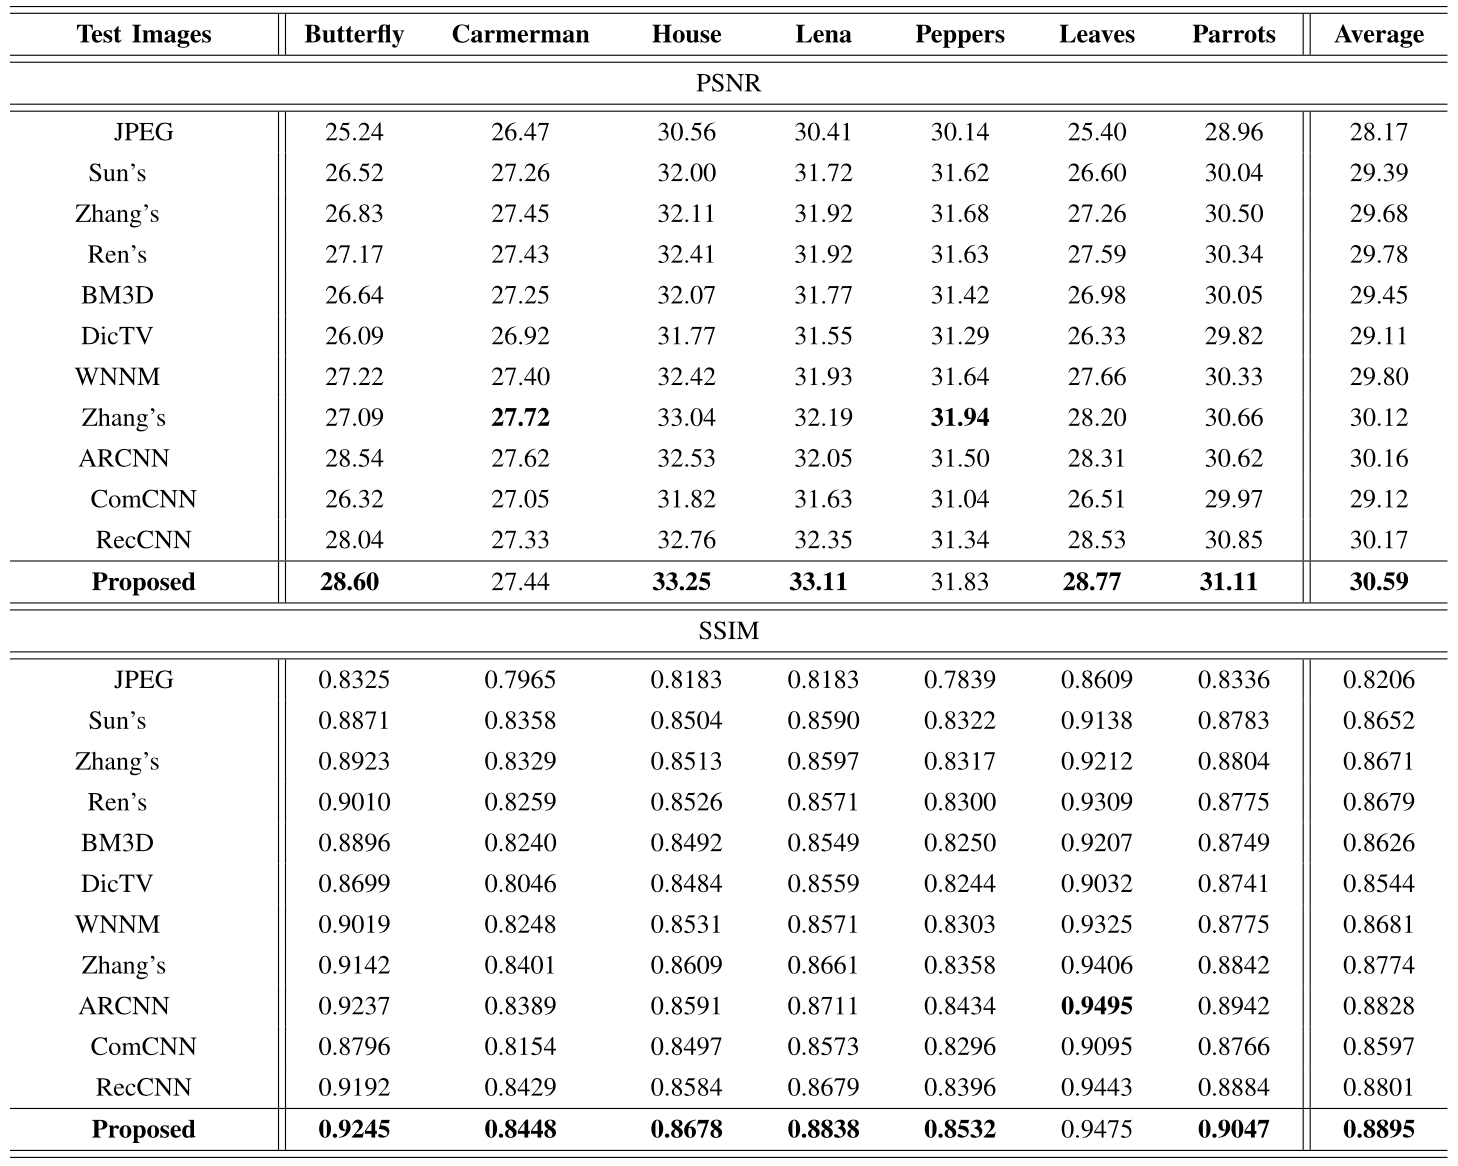
\includegraphics[width = 1 \linewidth]{images/paper3/comparison2.png}
                \caption{QF = 10, PSNR(db) and SSIM results of alghoritms image deblocking and denoising}
                \centering
            \end{figure}
        \end{minipage}
    \end{minipage}
\end{frame}

\begin{frame}{EXPERIMENTS: JPEG2000 vs. The proposed system}
    As we can see from the comparison made in figure \ref{fig:parrot}, the difference in  
    visual quality between the proposed method and the JPEG2000 codec is 
    considerable. With the same amount of bit rates, the JPEG2000 codec 
    produces worse results by losing several structural information. 
    \begin{minipage}{\linewidth}
        \centering
        \begin{minipage}{0.45\linewidth}
            \begin{figure}[H]
                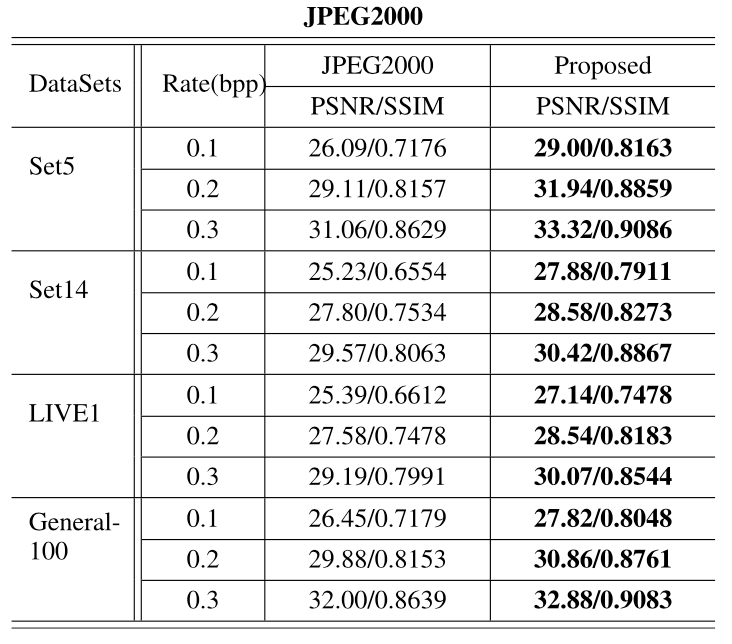
\includegraphics[width = 1 \linewidth]{images/paper3/JPEG2000.png}                
                \caption{Average PSNR(dB)/SSIM results of JPEG2000 and the proposed method on different datasets.}
            \end{figure}
        \end{minipage}
        \hspace{0.05\linewidth}
        \begin{minipage}{0.45\linewidth}
            \begin{figure}[htbp]
                \centering
                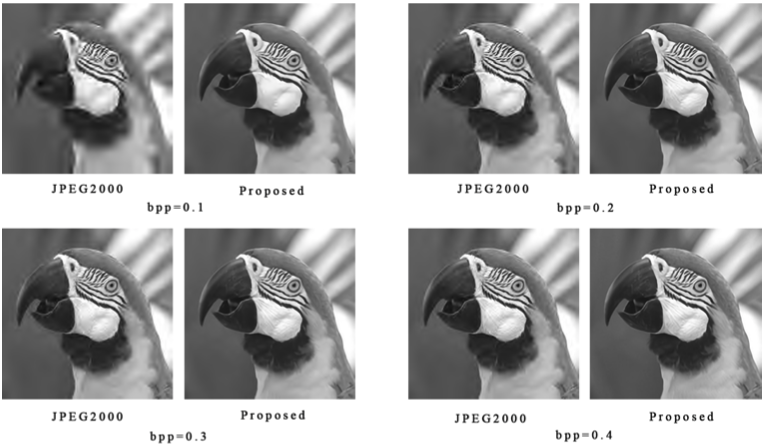
\includegraphics[width = 1 \linewidth]{images/paper3/JPEG2000p.png}
                \caption{Performance comparison of JPEG2000 at difference bit rates.}
                \label{fig:parrot}
                \centering
            \end{figure}
        \end{minipage}
    \end{minipage}
\end{frame}

\begin{frame}{EXPERIMENTS: BPG vs. The proposed system}
    As for the BPG codec, if used in combination with the \emph{ComCNN} and 
    \emph{RecCNN} networks, it reaches higher \emph{PSNR} and \emph{SSIM} levels than when 
    used individually or with only one of the two networks.   
    \begin{figure}[htbp]
        \centering
        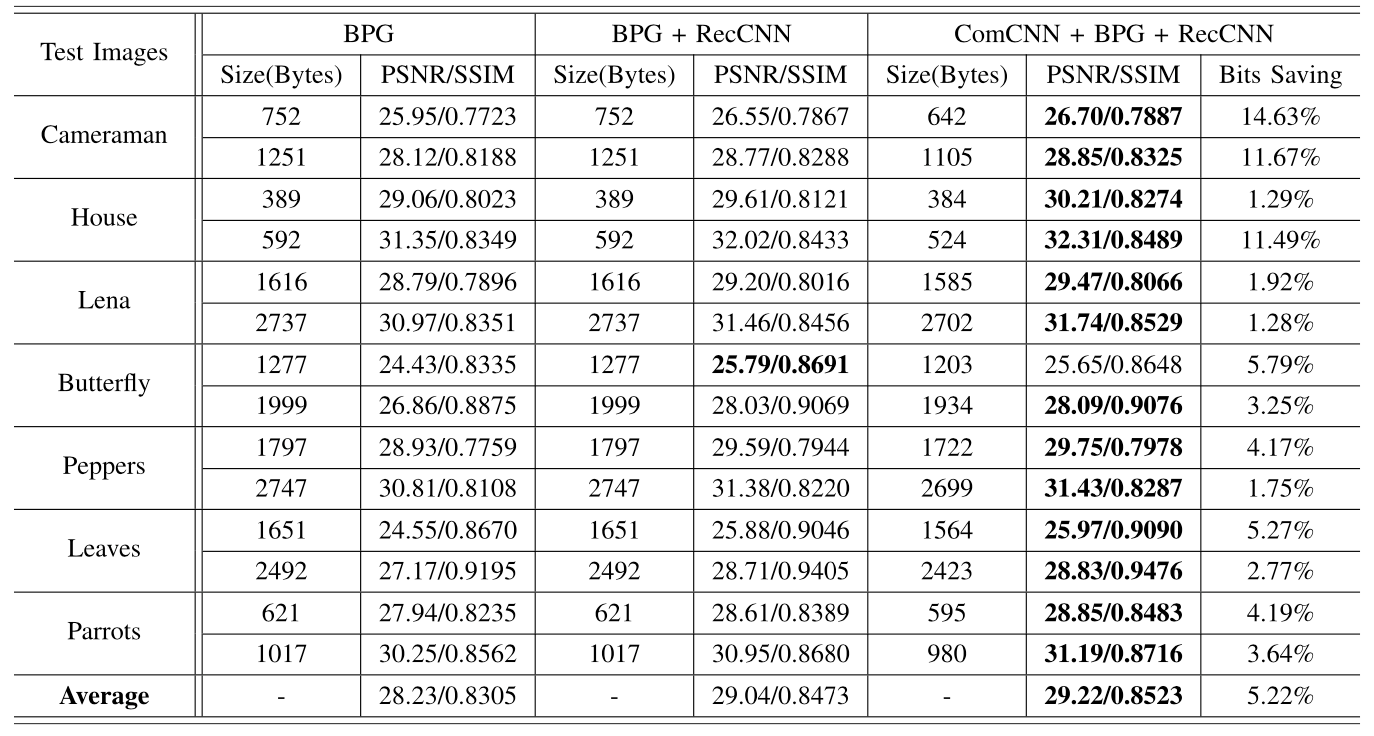
\includegraphics[width = 1 \linewidth]{images/paper3/BPG.png}
        \centering
        \caption{BPG: PSNR (dB) and SSIM result of BPG, BPG + RecCNN and the proposed method.}
        \label{fig:BPG}
    \end{figure}
\end{frame}

\begin{frame}{CONCLUSION}
    The proposed method seems to have the best performance compared to other 
    methods already existing in the state of the art. The proposed technique 
    then validates the use of one or more convolutional neural networks to carry 
    out the task of encoding and decoding images, even in some cases achieving 
    better quality than existing codecs for image compression.
    \begin{figure}[htbp]
        \centering
        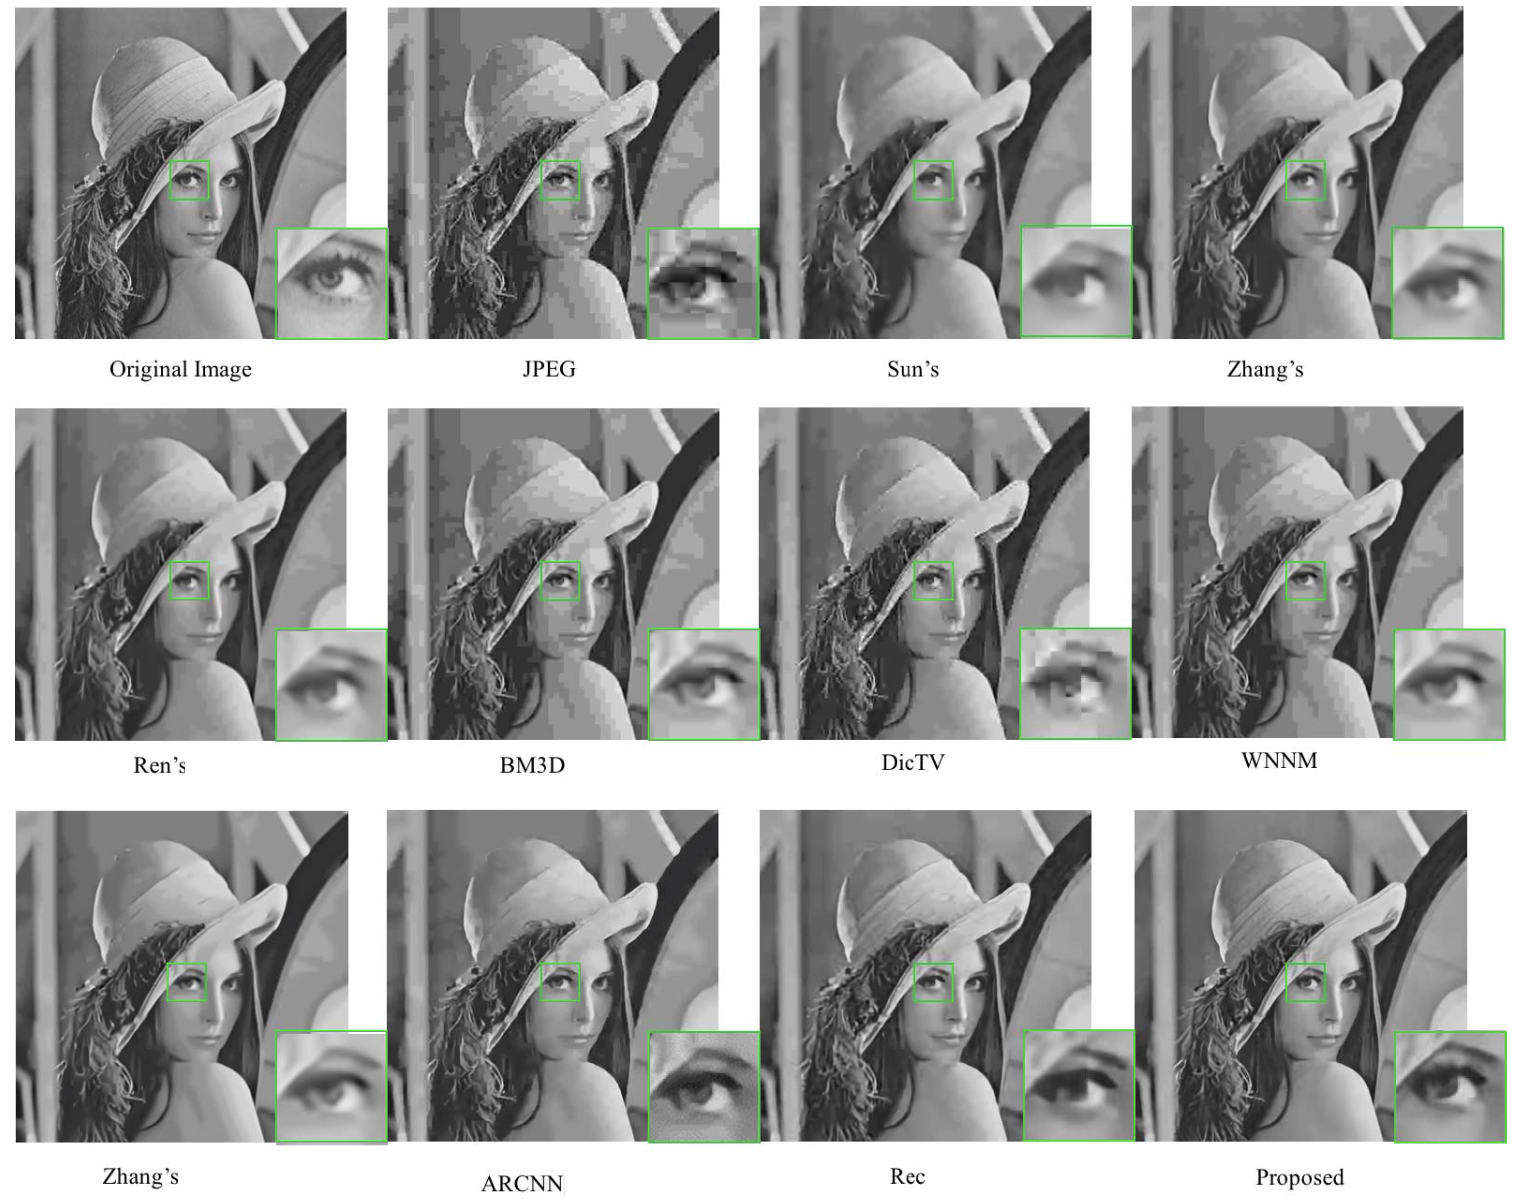
\includegraphics[width = 0.5 \linewidth]{images/paper3/final.png}
        \centering
        \caption{Visual quality comparison of image deblocking ad different QF.}
        \label{fig:final comparison}
    \end{figure}
\end{frame}